% Shared preamble for the English summaries in this repository.
\documentclass[11pt,a4paper]{article}
\usepackage[margin=2.2cm]{geometry}
\usepackage[T1]{fontenc}
\usepackage[utf8]{inputenc}
\usepackage{lmodern}
\usepackage{amsmath,amssymb}
\usepackage{graphicx}
\usepackage{booktabs}
\usepackage{enumitem}
\usepackage[hidelinks]{hyperref}
\setlist{itemsep=2pt,topsep=4pt}
\setlength{\parindent}{0pt}
\setlength{\parskip}{5pt}
\graphicspath{{figures/}}
\newcommand{\summaryheader}[3]{%
  \begin{center}
    {\Large\bfseries #2}\\[3pt]
    {\large #1}\\[3pt]
    {\small Arshia Goshtasbi \textbullet{} MSc Electrical Engineering (Control), Iran University of Science and Technology \textbullet{} #3}
  \end{center}
  \vspace{2pt}\hrule\vspace{8pt}
  \noindent\textit{English summary of my original Persian report, which is kept as a PDF in this folder.}\par}

\begin{document}
\summaryheader{Adaptive Control, Homework 3}{Indirect Self-tuning Regulators (Åström \& Wittenmark, Examples 3.4--3.6)}{Autumn 1404 (2025)}

All three cases are subsystems of \texttt{HW3.slx}. Each one combines RLS estimation of the plant with a pole-placement design recomputed at every step from the current estimates. For each case my report puts my simulation next to the book's figure: output tracking of a square-wave reference, the control signal, and the parameter estimates.

\begin{description}
  \item[Example 3.4: with zero cancellation.] The controller cancels the process zero.
  \item[Example 3.5: without zero cancellation.] The process zero is kept in the closed-loop response.
  \item[Example 3.6: continuous-time STR.] The same design applied to a continuous-time plant model.
\end{description}

\begin{center}
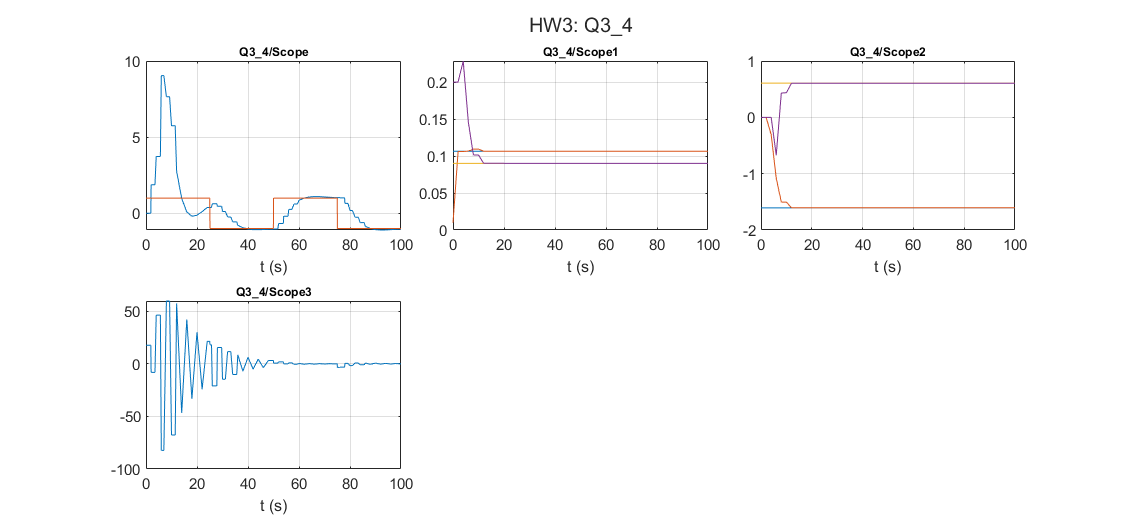
\includegraphics[width=0.9\linewidth]{Q3_4.png}\\[2pt]
{\small Re-run in R2023b: example 3.4, output and reference, estimates and control signal.}
\end{center}
\end{document}
